\documentclass[10pt, a4paper, onesided]{article}

\usepackage{dingbat}
\usepackage{graphicx}
\usepackage{enumitem}
\renewcommand{\familydefault}{\sfdefault}
\usepackage[colorlinks=false]{hyperref}

\usepackage{listings}
\lstset{basicstyle=\small\ttfamily,breaklines=true}

\setlength{\parskip}{6pt}
\setlength{\parindent}{0pt}

%opening
\title{\textbf{clickyBoard} Documentation}
\author{}
\date{}

\begin{document}
\maketitle
\vspace{-60pt}

\begin{center}
	\textit{For board version 1.1}
\end{center}
\vspace{-12pt}
Download this document at \href{https://github.com/SecretImbecile/clickyBoard}{github.com/SecretImbecile/clickyBoard}
\tableofcontents

\section{The clickyBoard}

	The \textit{clickyBoard} is an add-on board for the Raspberry Pi computer (model B+ or later), which adds a simple switch and LED circuit for use in GPIO programming.
	
	The clickyBoard has been designed to use Cherry MX series switches or compatible switches from other manufacturers, designed for use in keyboards that are widely available and cheaply purchased.
	
	The board, through the Raspberry PI GPIO, provides four push-buttons inputs, as well as a single output through which you can control the four backlight LEDs under each key.
	
	In addition to technical documentation, this document also includes a parts list and assembly guide, for users wishing to assemble their own clickyBoard from scratch, or kit form.

\newpage
\section{Parts Required}

	The following components are required to fully populate a clickyBoard:
	
	\begin{itemize}[noitemsep]
		\item two $1 k\Omega$ resistors
		\item four T1 (3mm) LEDs
		\item four resistors, of a value determined in \autoref{LEDresistors}
		\item one TO-220 package logic level power MOSFET
		\item four Cherry MX compatible switches
		\item a female 40-pin connector for the Raspberry Pi GPIO header\footnote{a $2\times20$ header with $2.54 mm$ ($0.1"$) pitch}
	\end{itemize}
	
	\subsection{Mechanical Keyboard Switches}
	
	The clickyBoard has mounting holes for MX series or compatible switches. These are switches designed for use in premium computer keyboards, which are widely available, along with compatible keycaps.
	
	\begin{figure}[h]
		\centering
		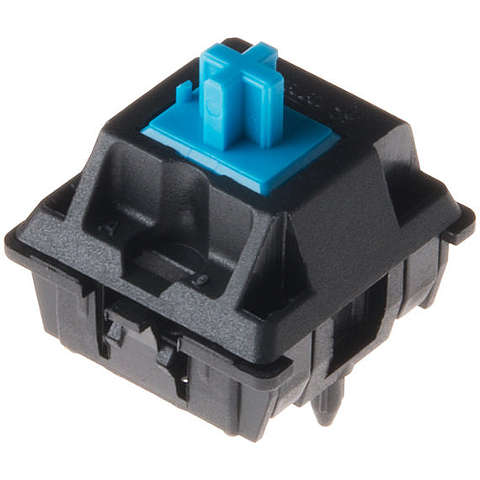
\includegraphics[width=0.25\linewidth]{img/cherrymx}
		\caption{A Cherry MX Blue switch}
		\label{fig:cherrymx}
	\end{figure}
	
	If you require quick delivery, the german manufactured \textbf{Cherry MX} series of switches are more readily available from several on-line retailers. In the United Kingdom, one possibility would be a computer hardware retailer like \href{http://www.kustompcs.co.uk/acatalog/Keys_and_Accessories.html}{kustompcs.co.uk}. In the US and internationally, \href{http://www.wasdkeyboards.com/index.php/products/keyboard-parts.html}{wasdkeyboards.com} specialises in mechanical keyboard parts. Cherry switches are likely to cost around \pounds1 per switch.
	
	If you're willing to wait for shipping from China, there are several manufacturers that make compatible switches, notably \textbf{Gateron} and \textit{Kailh} switches. Gateron switches can be purchased on eBay for as little as 10 for \pounds1.
	
	There are several types of MX switch available, denoted by the colour of their centre plunger, as shown in \autoref*{fig:cherrymx}. We recommend \textbf{blue} coloured switches, for full authentic clickiness, but others are available.
	
	If possible, opt for `\textbf{PCB mount}' switches (sometimes referred to as `5-pin'), as these have additional plastic pegs which will ensure the switches are correctly oriented. Using `plate mount' switches will usually result in slightly misaligned switches.
	
	\begin{center}
	\begin{tabular}{c|c|c|c}
		Switch Colour & Click & Tactile Bump & Heavy Spring \\ 
		\hline 
		Blue & \checkmark & \checkmark & \\ 
		Green & \checkmark & \checkmark & \checkmark \\ 
		Brown &  & \checkmark & \\ 
		Clear &  & \checkmark & \checkmark \\ 
		Red &  &  & \\ 
		Black &  &  & \checkmark \\ 
	\end{tabular}
	\end{center}

	
	
	\subsection{LED and Resistor Choice}
	\label{LEDresistors}

	To fit within the housing of an MX compatible switch, a 3mm (T1) LED must be chosen.
	
	To provide sufficient current, the LEDs on the clickyBoard are powered through the Raspberry Pi's 5 volt supply, rather than the current-limited 3V3 GPIO pins, and are instead controlled using a power MOSFET and a single GPIO output.
	
	Each LED has a resistor in series. The required resistance for the circuit can be calculated using this variant of the standard resistance formula, where $V_s$ is the supply voltage, and $V_f$ is the forward voltage of the chosen LED.
	
	\begin{displaymath}
		R = \frac{V_s - V_f}{I}
	\end{displaymath}
	
	For the red $2 V$ $20 mA$ LEDs used in the schematic, the resistance for the LED resistors was calculated as follows.
	
	\begin{displaymath}
		R = \frac{5 V - 2 V}{20 \times 10^{-3} A} = 150 \Omega
	\end{displaymath}

\newpage
\section{Assembly Guide}

	\subsection*{Soldering Basics}
		This guide will assume that the reader is familiar with basic soldering techniques. The components on the clickyBoard are all through-hole components, so it may be a suitable board for a novice solderer. Be aware that the 40-pin GPIO header can be tricky, especially with an old soldering iron, or thick gauge solder wire.
		
		With that said, here are some resources for learning to solder. Video tutorials are well suited for soldering, as you'll need to be able to identify a good solder joint from a bad one.
		\begin{itemize}[nolistsep]
			\item \textit{Soldering basics and choosing a cheap soldering iron} (00:00--12:00), bigclivedotcom --- \url{https://www.youtube.com/watch?v=aIab66EgfHM}
			\item \textit{EEVblog \#183 - Soldering Tutorial Part 2}, EEVblog --- \url{https://www.youtube.com/watch?v=fYz5nIHH0iY}
		\end{itemize}
	
	\subsection*{Resistors}
	
		For convenience, we always solder components from lowest height to highest, to maintain a steady PCB on which to work. Begin by soldering the two $1 k\Omega$ resistors in slots \texttt{r1} and \texttt{r2}.
		
		Next, solder the resistors for the LEDs that you chose in \autoref{LEDresistors} into the sockets \texttt{r3}--\texttt{r6}.
	
	\subsection*{MOSFET}
	
		Bend the legs of your TO-220 package MOSFET to a 90 degree angle and place it in the socket so that the large metal tab is flush with the PCB. You can optionally solder the tab to the large pad on the board, then solder the three main pins into their holes.
		
		If you are \textbf{not} using a MOSFET to control the LEDs, you should jumper the two topmost pins, either by bridging the holes with solder, or with a piece of wire.
	
	\subsection*{Switches \& LEDs}
	
		\subsubsection*{Switch assembly}
	
			In MX style switches, the 3mm LED sits in a slot at the bottom of the switch, and the leads are fed through holes in the switch housing. It is recommended to place the LED in the switch, then inserting that complete assembly into the board to solder.
			
			Ensure that the polarity of the LED is correct, and the switch is sitting flush with the board with the plastic peg(s) in their respective holes, then solder the connections of both the switch and LED.
	
	\subsection*{40-pin GPIO header}
	
		To complete the \textit{clickyBoard}, solder the 40-pin female header to the board, with the female socket on the reverse side of the board.
		
		If you choose not to solder all of the pins, the following pins are required (GPIO board pinout numbering): 
		\texttt{1 4 9 11 12 13 15 16}, omitting \texttt{11} if a MOSFET was not used.


\newpage
\section{Example Code}

The clickyBoard provides the following GPIO devices (all pins are GPIO board numbers):

\begin{itemize}[nosep]
	\item LED brightness control through pin \textbf{11}
	\item switch inputs through pins \textbf{12}, \textbf{13}, \textbf{15}, and \textbf{16}
\end{itemize}

The switch inputs require the internal GPIO pull-down resistors in the Raspberry Pi to be enabled. enable them by setting up the pins with the \texttt{pull\_up\_down} parameter set to \texttt{GPIO.PUD\_DOWN}.

The following example Python program will demonstrate the functionality of the clickyBoard. (note that \texttt{GPIO.cleanup()} is not run following this program)

\begin{lstlisting}[language=Python,title=clickyboardtest.py,numbers=left]
import RPi.GPIO as GPIO
import time

# Setup Pins
GPIO.setmode(GPIO.BOARD)

GPIO.setup(11, GPIO.OUT)
GPIO.setup(12, GPIO.IN, pull_up_down=GPIO.PUD_DOWN)
GPIO.setup(13, GPIO.IN, pull_up_down=GPIO.PUD_DOWN)
GPIO.setup(15, GPIO.IN, pull_up_down=GPIO.PUD_DOWN)
GPIO.setup(16, GPIO.IN, pull_up_down=GPIO.PUD_DOWN)

# Setup Backlight
pwm = GPIO.PWM(11, 60)
pwm.start(100)

while True:
	#Create a count of the buttons being pressed
	buttons_pressed = 0
	
	if GPIO.input(12) == GPIO.HIGH:
		buttons_pressed += 1
	if GPIO.input(13) == GPIO.HIGH:
		buttons_pressed += 1
	if GPIO.input(15) == GPIO.HIGH:
		buttons_pressed += 1
	if GPIO.input(16) == GPIO.HIGH:
		buttons_pressed += 1
	
	#Reduce PWM brightness based on number of buttons
	pwm.ChangeDutyCycle(100 - (25 * buttons_pressed))
	
	time.sleep(0.1)
	
\end{lstlisting}

\newpage
\section{Technical Documentation}
	\subsection{Schematic design for the clickyBoard}
		\begin{center}
			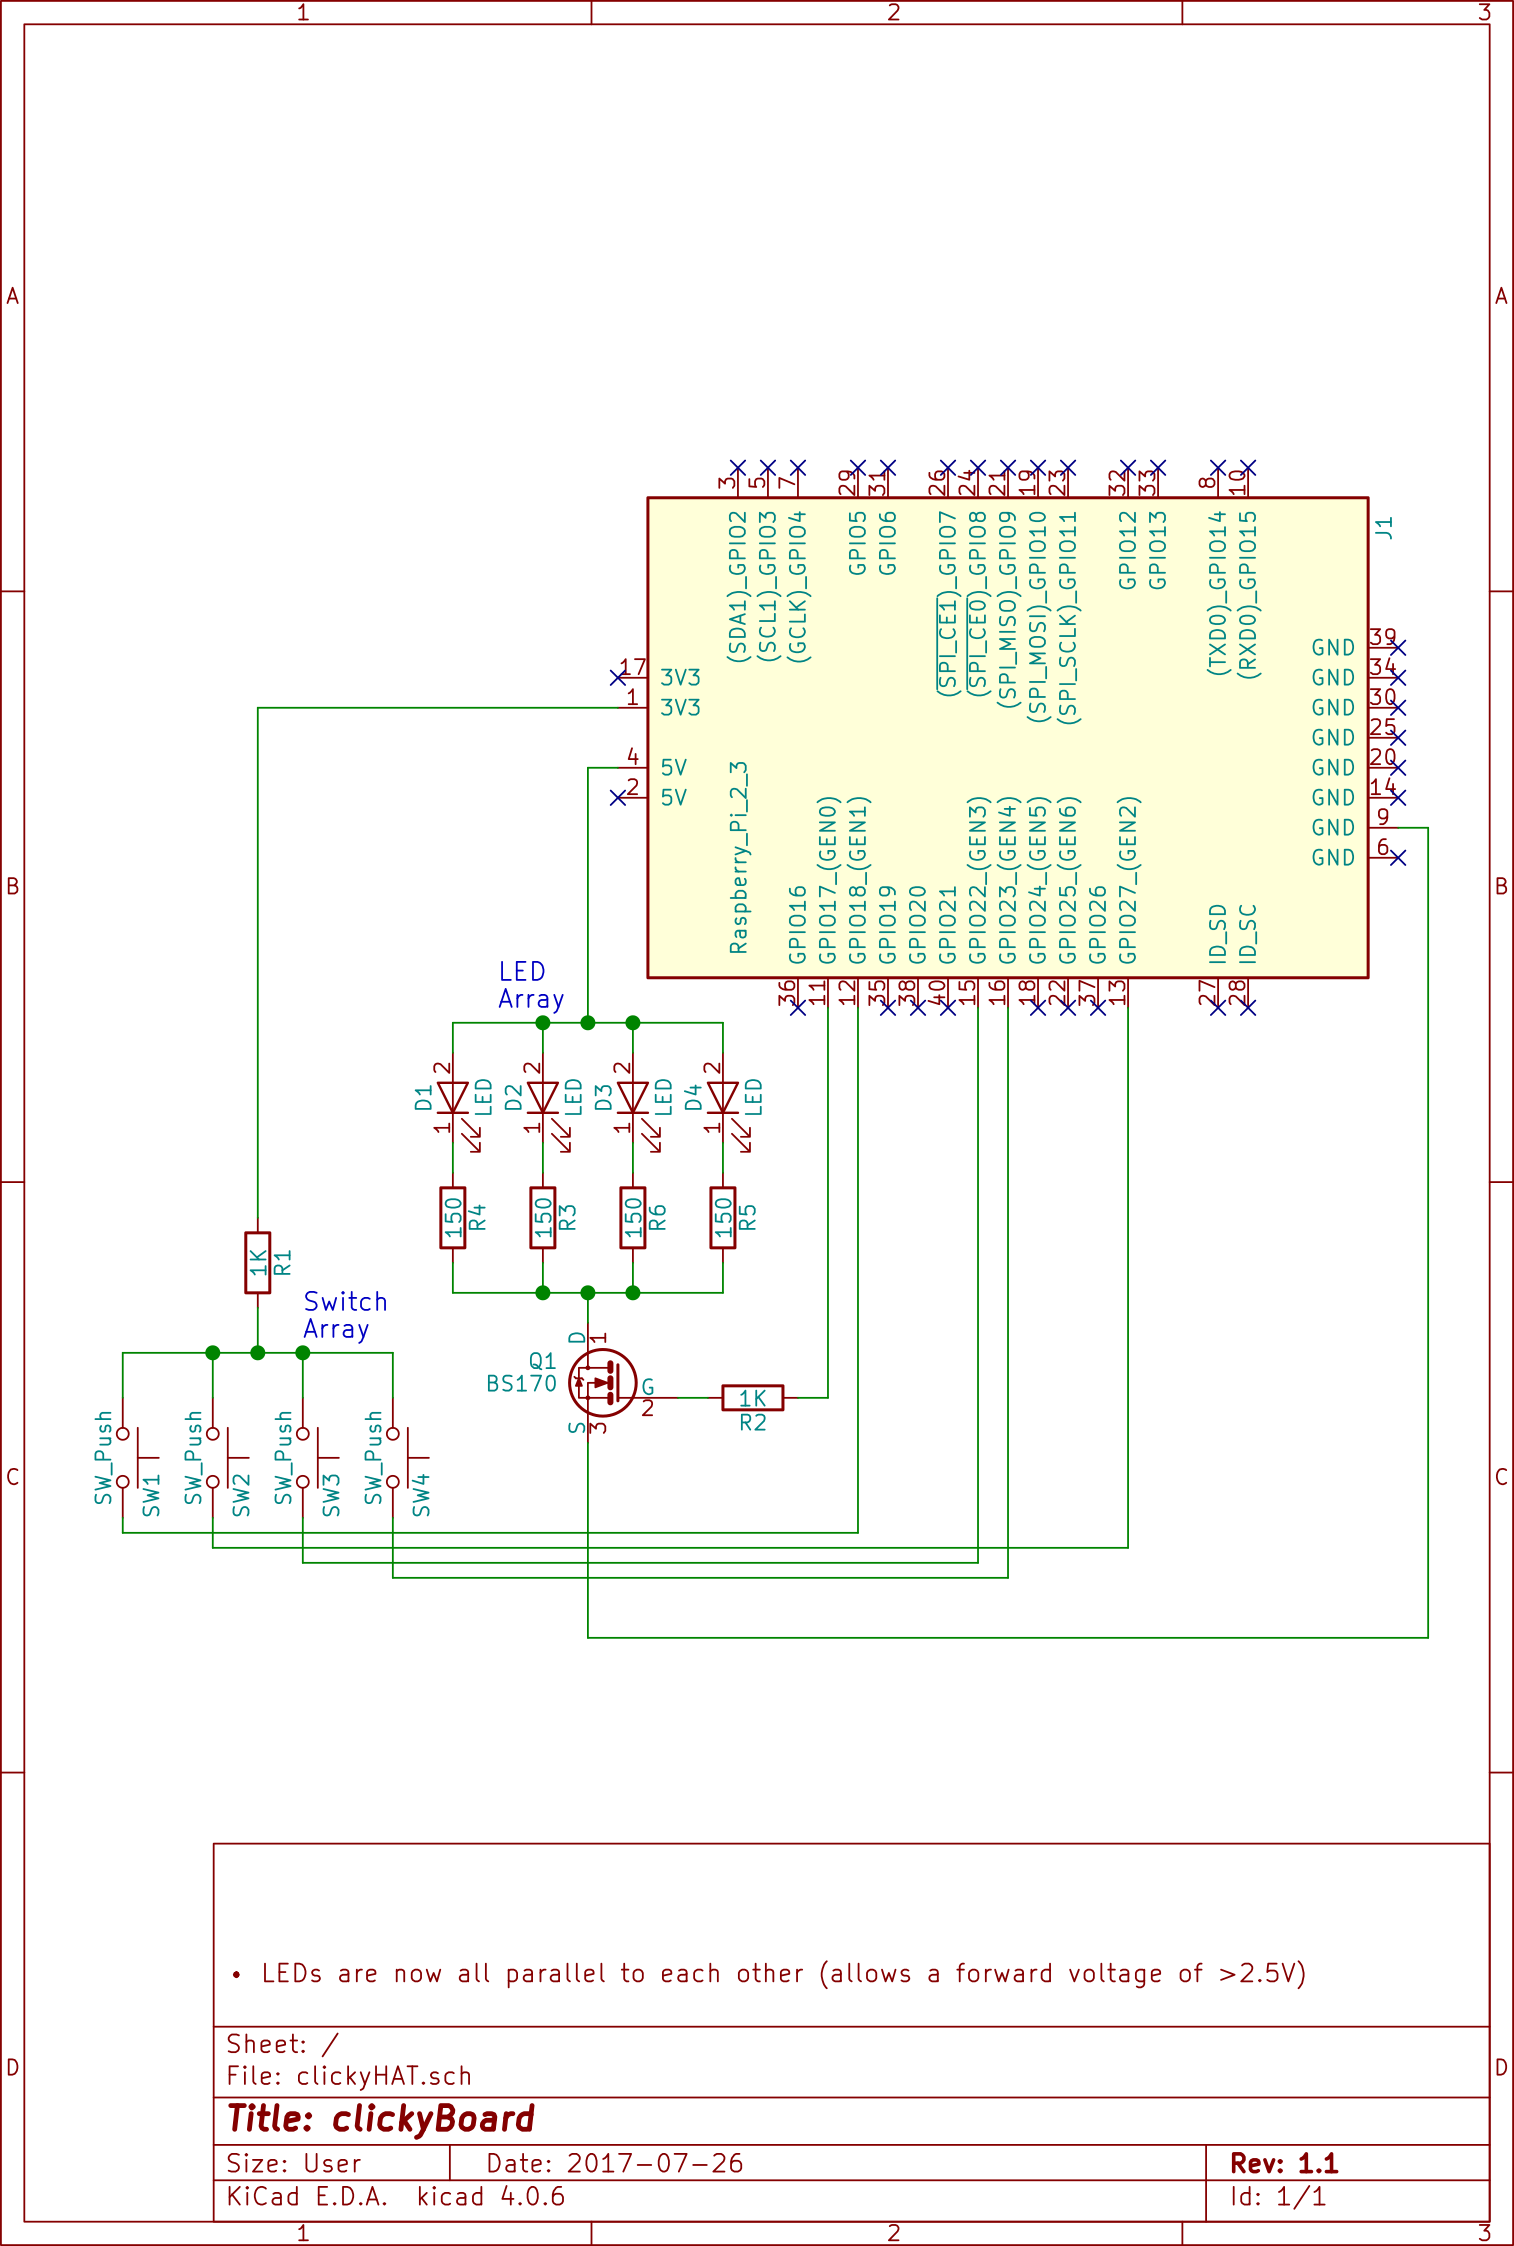
\includegraphics[width=1\linewidth]{img/schematic}
		\end{center}
	
	\newpage
	\subsection{PCB layout for the clickyBoard}
		Gerber outputs (with additional layers) are available on the \href{https://github.com/SecretImbecile/clickyBoard}{GitHub repo}.
		\subsubsection*{Front Copper}
			\begin{center}
				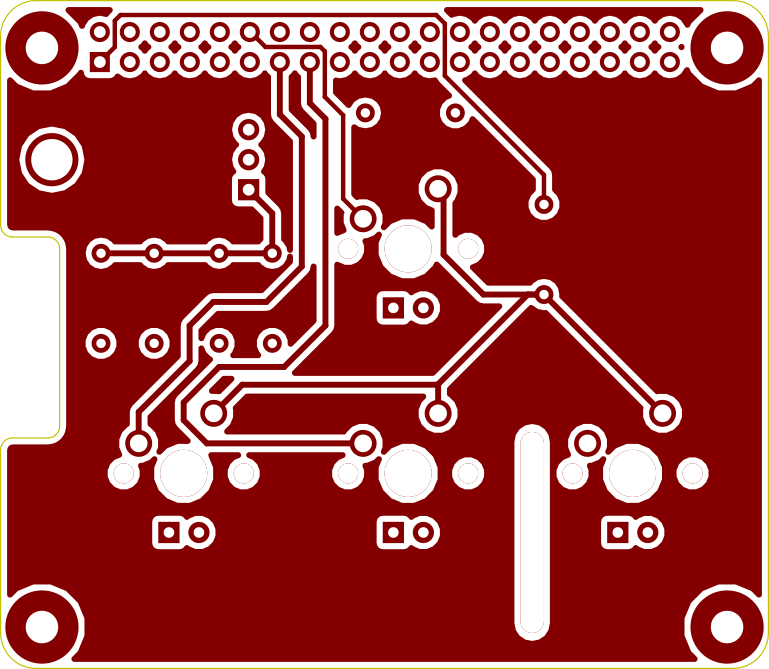
\includegraphics[width=0.7\linewidth]{img/F_Cu}
			\end{center}
		\subsubsection*{Back Copper}
		\begin{center}
			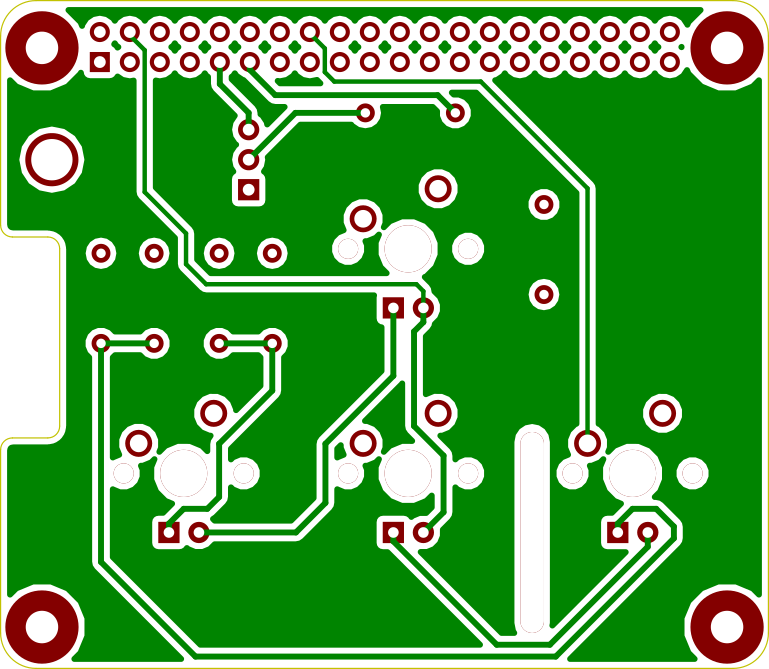
\includegraphics[width=0.7\linewidth]{img/B_Cu}
		\end{center}
		\subsubsection*{Front Silkscreen}
		\begin{center}
			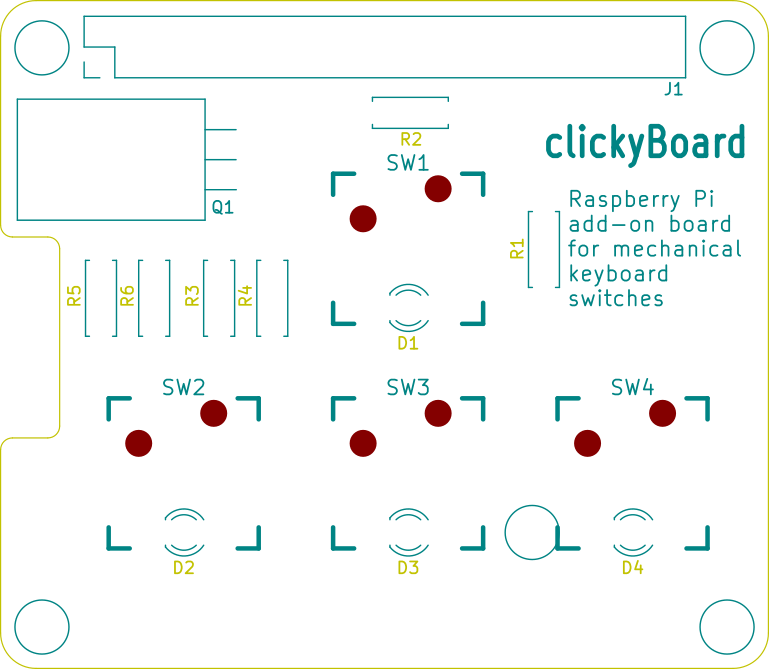
\includegraphics[width=0.7\linewidth]{img/F_Ss}
		\end{center}
	
	\subsection*{Design rules for PCB}

		The design rules used for this PCB were as follows.
	
		\begin{tabular}{c|c|c|c}
			Clearance & Track Width & Via Size & Silkscreen line thickness \\ 
			\hline 
			$0.2 mm$ & $\ge 0.375 mm$ & n/a & $\ge 0.15 mm$ \\ 
		\end{tabular}

\iffalse
	\subsection{Board errors in version 1.0}
	
		\subsubsection*{MOSFET miswiring}
		\label{MOSFETerror}
		
		Note that the mosfet pads are miswired on version 1.0, and the mosfet should be manually corrected with jumper wires. This has been rectified in version 1.1.
	
		\subsubsection*{LED pad direction}
		\label{LEDerror}
		
		Please note that the solder pads for the LEDs are reversed on board version 1.0. This has been rectified in version 1.1.
		
		By convention, the square solder pad indicates the positive side of a diode. However, because of an update to the \textit{KiCad} software, the pins in the component library were reversed. You should therefore solder the (longer) \textbf{positive} lead of the LEDs into the \textbf{circular} pads. 
		
		\begin{quote}
			\textit{...all diodes in KiCad's standard libraries have seen their pin numbers swapped. This is to be in line with most other software and the IPC standard as well, which states that cathode should be pin 1.}\footnote{\url{https://forum.kicad.info/t/important-announcement-diode-pins-swapped-in-standard-kicad-libraries/820}}
		\end{quote}
	
		\subsubsection*{LED array voltage}
		\label{LEDerror2}
		
		Due to the series arrangement of the LEDs in board version 1.0, blue LEDs would not be useable, this has been rectified in version 1.1.
		
		LEDs were arranged into 2 parallel series as shown in \autoref{fig:documentation}, providing each LED a maximum voltage of 2.5V. Because blue LEDs require a higher forward voltage, most blue and white LEDs will not work on version 1.0 of the clickyBoard, limiting you to red, yellow or green backlighting for most LEDs.
\fi

\newpage
\section{License}

	The complete hardware design for the clickyBoard, including the files made available on the clickyBoard \href{https://github.com/SecretImbecile/clickyBoard}{GitHub repo} and all documentation, are released in accordance with the \href{https://www.oshwa.org/definition/}{Open Source Hardware (OSHW) Definition}, under the \href{https://creativecommons.org/licenses/by-sa/4.0/}{\textbf{Creative Commons Attribution-ShareAlike 4.0 International (CC BY-SA 4.0)}} license.
	
	Every effort has been made to comply with the OSHW statement of principles. If you feel any aspect of the OSHW priciples have been neglected, please raise the issue with the creator (a GitHub issue report would be suitable).
\end{document}
